\documentclass{template/openetcs_article}
%\documentclass{article}
%\usepackage[ascii]{inputenc}
%\usepackage[T1]{fontenc}
\usepackage[english]{babel}
\usepackage{amsmath}
\usepackage{amssymb,amsfonts,textcomp}
\usepackage{array}
\usepackage{supertabular}
\usepackage{hhline}
\usepackage{graphicx}
\makeatletter
\newcommand\arraybslash{\let\\\@arraycr}
\makeatother
\setlength\tabcolsep{1mm}
\renewcommand\arraystretch{1.3}
\newcounter{Ilustracin}
\renewcommand\theIlustracin{\arabic{Ilustracin}}
\title{openETCS}

%\setcounter{tocdepth}{3}
\usepackage{float}
\usepackage{hhline}
\usepackage{booktabs}
\usepackage{multirow}
\usepackage{color, colortbl}
\definecolor{myblue}{rgb}{0.6,.6,1}
\definecolor{mydarkblue}{rgb}{0,0,0.5}
\definecolor{mylightblue}{rgb}{0.8,0.8,1}
\usepackage{hyperref}
\hypersetup{colorlinks=true, linkcolor=mydarkblue, urlcolor=mydarkblue}

\usepackage[textwidth=2.7cm,textsize=scriptsize,linecolor=green!40,backgroundcolor=green!40]{todonotes}

\newcounter{mycommentcounter}
\newcommand{\mycomment}[2][]
{
\refstepcounter{mycommentcounter}%
\todo[color={red!100!green!33}]{
\textbf{[\uppercase{#1} \themycommentcounter]:} #2}
}


\usepackage{lipsum,url}
\graphicspath{{./template/}{.}{./images/}}
\begin{document}
\frontmatter
\project{openETCS}

%Please do not change anything above this line
%============================
% The document metadata is defined below

%assign a report number here
\reportnum{OETCS/WP1/D1.3.1}

%define your workpackage here
\wp{Work-Package 1: ``Management''}

%set a title here
\title{Project Quality Assurance Plan - Revision Process}

%set a subtitle here
%\subtitle{A template for short document. Adapted from report template.}

%set the date of the report here
\date{\today}

%define a list of authors and their affiliation here

\author{SQS}

\affiliation{Avda. Zugazarte 8,6\\
  48930 Getxo \\
  Vizcaya, España}


% define the coverart
\coverart[width=350pt]{openETCS_EUPL}

%define the type of report
\reporttype{Description of work}




%=============================
%Do not change the next three lines
\maketitle
\tableofcontents
%\listoffiguresandtables
\newpage
%=============================

% The actual document starts below this line
%=============================


%Start here



%\begin{document}


\section*{Document History}

\begin{flushleft}
%\tablefirsthead{\hline Version & Date & Chapters modified & Reason & Name\\}

\tablehead{\hline \rowcolor{myblue} Version & Date & Chapters modified & Reason & Name\\}

\tabletail{}
\tablelasttail{}
\begin{supertabular}{m{1.1cm}m{1.8cm}m{2cm}m{7cm}m{2cm}lp{6cm}|}
\hline
0.0.1 &
09.04.2013 &
All &
First version &
SQS
\\\hline
0.0.2 &
12.04.2013 &
Roles &
Tables added to the 'Roles' section &
SQS
\\\hline
0.0.3 &
15.04.2013 &
T.instructions &
Technical instructions completed &
SQS
\\\hline
0.0.4 &
16.05.2013 &
All &
Comments of the reviewers analysed and some changes implemented &
SQS
\\\hline
0.0.5 &
23.05.2013 &
All &
New complete version adjusted to the Revision process concept &
SQS
\end{supertabular}
\end{flushleft}

\newpage

\section{Introduction}

\subsection[Introduction]{Purpose of the document}
This document presents the whole process to follow when documents need revision. It aims to provide a set of guidelines as technical instructions for each revision cycle launched that highlights the steps to take.The roles involved in the process are clearly identified as well as their responsibilities and tasks. And finally, the mechanisms needed to achieve the proposed objectives are also included, so the process can be carried out successfully.

\subsection{Intended Audience}
This document applies to the whole development life-cycle of the project and it addresses all the author(s) and committers involved. This document should be available to all of them in read access mode and it provides guidance about the Revision process to follow anytime revisions of documents are needed.

\subsection{Supporting documents}
\tablefirsthead{\hline
\rowcolor{myblue}
Name &
Path &
Contents\\}
\tablehead{}
\tabletail{}
\tablelasttail{}
\begin{supertabular}{|m{2cm}m{3cm}m{9cm}|}
\hline
Todonotes package &
governance/Review Process &
Brief introduction to the todonotes package with detailed descriptions about the available attributes. 
\\\hline
\end{supertabular}

\subsection{Definitions and acronyms}
\tablefirsthead{\hline
\rowcolor{myblue}
Abbreviation &
Meaning\\}
\tablehead{}
\tabletail{}
\tablelasttail{}
\begin{supertabular}{|m{3cm}m{11cm}|}
\hline
Revision Process &
The OpenETCS committers are invited to perform a revision of the contents of a document. The committers can edit the document, writing complete sections or making changes directly in it (LaTex, todonotes and Smartgit tools). The author(s) shall support the whole process answering questions and resolving conflicts. Once the author(s) and committers are satisfied with the results, the Product owner shall confirm and approve or reject and request more changes to the revised document. Finally, the approved document is pushed into the corresponding GitHub repository.
\\\hline
Review Process &
Any person involved in the GitHub communnity and/or the OpenETCS project is invited to participate in a Review Process. They shall not edit the document but send comments and suggestions creating the corresponding issues in the {\it Issue Tracker} tool. Once the deadline has arrived, the author(s) shall collect the comments and make the changes they consider appropriate. Any doubt shall be answered by the reviewers using the issue threads opened and in case of conflicts the collaboration of the Product owner may be required. The process may be launched after a Revision Process ends, there are relevant issues reported for a release or whenever the Product owner considers appropriate. 
\\\hline
RC &
Revision Cycle - A complete cycle with an established deadline (one or two weeks maximum) where the author(s) and the committers can read, analyse and make suggestions or changes directly to the document under revision. Once the document is approved the cycle finishes and a new version shall be available in the corresponding GitHub repository.
\\\hline
Product owner &
The role played by the main author of a document or the project leader. The responsibilities of the role include launching a Revision process, inviting committers to the process, closing discussions, taking decisions when there are conflicts and doing the final approval of the document among others.
\\\hline
Committer &
The role played by a member of the OpenETCS project who have been granted with this role by other committers and the project leader. There are some tasks that only can be done by committers such as: editing and pushing changes or new documents into a GitHub repository, closing of issues in the {\it Issue Tracker} or being involved in Revision processes.
   
\end{supertabular}

\section{Tools}

\begin{flushleft}

\begin{tabular}{|m{3cm}|m{11cm}|}
\hline
\rowcolor{myblue}
\multicolumn{2}{|c|}{Tools} \\\hline
GIT &
\begin{itemize}
\item GitHub: A web-based hosting service for projects that use Git revision control system.
\item SmartGit: A graphical front-end for Git distributed version control systems. 
\end{itemize}\\\hline
Pdf documents &
\begin{itemize}
\item Adobe Acrobat Reader: Software package that allows to view, navigate and print pdf files.
\item Diffpdf: Open source application that compares different PDF files for discrepancies. 
\item {PDF Creator: Software for creating pdf files. Works like a printer on your PC.}
\end{itemize}\\\hline
TeX documents &
\begin{itemize}
\item MiKTeX : Provides the tools necessary to prepare documents using de TeX/LaTeX mark up language.
\item GhostScript. 
\item GhostView.
\item TexMaker.
\item Todonotes package.
\item Adobe Acrobat Reader: Software package that allows to view, navigate and print pdf files.
\end{itemize}\\\hline
\end{tabular}
\end{flushleft}

\section{Revision Process overview}
\subsection{Structure of the repository}
 
The Revision process involves the creation of the following directory inside the structure of each repository once a {\it new branch} for the revision has been created.

\begin{flushleft}
\begin{tabular}{|m{3cm}|m{11cm}|}
\hline
\rowcolor{myblue}
\multicolumn{2}{|c|}{Structure of the repository} \\\hline
\rowcolor{lightgray}
Name &
Content 
\\\hline
Revision Documents &
\begin{itemize}
\item The document under revision: In Tex and PDF formats with all its history of changes, comments and sections added.
\end{itemize}\\\hline
\end{tabular}
\end{flushleft}

\subsection{Revision Roles}

This section describes the roles of the participants in the revision process of a document:

\begin{flushleft}
\begin{tabular}{|m{3cm}|m{11cm}|}
\hline
\rowcolor{myblue}
\multicolumn{2}{|c|}{Roles} \\\hline
\rowcolor{lightgray}
Role &
Competencies \\\hline
Product owner (main author or project leader) &
\begin{itemize}
\item Launch the Revision Process.
\item Open a Revision cycle for a document creating a git new branch ({\it TI.1.1. New RC branch}) 
\item Notify the Committers via a personal e-mail or opening a new issue.  ({\it TI.1.2. Invite Committers})
\end{itemize}
\item Control Revision Process ({\it TI.1.3. Supervision of the Revision Process})
\begin{itemize}
\item Approve the revised version and confirmation of changes made ({\it TI.1.4. Final approval and confirmation of the revised version})
\item Send the notification of closing. ({\it TI.1.5. Revision closing})
\item Merge the associated RC branch into the repository master branch. ({\it TI.1.6. RC Branch merging})
\item Generate an established version of the document and pushed it in the corresponding GitHub repository. ({\it LaTex and PDF versions})
\end{itemize}
\\\\\hline
\end{tabular}
\end{flushleft}

\begin{flushleft}
\begin{tabular}{|m{3cm}|m{11cm}|}
\hline
\rowcolor{myblue}
\multicolumn{2}{|c|}{Roles} \\\hline
\rowcolor{lightgray}
Role &
Competencies \\\hline
Author(s) & 
\begin{itemize}
\item Supervision of the work being done. 
\begin{itemize}
\item Use todonotes tool to add, verify and reject comments in the document being reviewed. ({\it TI.2.1. Approval/rejection of comments})
\item Make changes to the document when required.
\item Make a request to the product owner for a final confirmation of the changes made. 
\end{itemize}
\end{itemize}
\\\\\hline
\end{tabular}
\end{flushleft}

\begin{flushleft}
\begin{tabular}{|m{3cm}|m{11cm}|}
\hline
\rowcolor{myblue}
\multicolumn{2}{|c|}{Roles} \\\hline
\rowcolor{lightgray}
Role &
competencies 
\\\hline
Committers &
\begin{itemize}
\item Confirm the participation in the Revision. Justify the no involvement in any other case.
\item Prepare the working environment: the committer clones the repository in local, creates a branch and associates it to the repository on GitHub ({\it TI.3.1. Revision environment setup}).
\item Be aware of how to perform the revision work ({\it TI.3.2 Revision work})
\begin{itemize}
\item Make comments, suggestions or improvement proposals with the todonotes package installed for the LaTeX editing tool. ({\it TI.4.2 Add notes using todonotes})
\item Work directly in the document, adding texts and sections. 
\item Send comments in case of conflicts or doubts to the author(s) through the {\it Issue Tracker} or e-mail.
\end{itemize}
\end{itemize}
\\\hline
\end{tabular}
\end{flushleft}

\subsection{Description of the Revision Process}

This subject is concerned with the validation and verification of the documentation generated within the OpenETCS project. The process shall aim to confirm that what has been produced is correct and meets the expectations of the committers as well as improving the quality of the document and its reliability; it also ensures the technical approach is appropriate before releasing the related documentation.

A Revision Cycle will help the project to better meet its strategic goals and objectives, so the correctness of the deliverables is ensured and they cover their intended purpose.The following aspects shall be assessed during the Revision Process:

\begin{itemize}
\item The material is technically accurate
\item The goals of the document have been achieved
\item Quality, style and grammar (do not forget the spell check)
\item Document uses consistent tense
\item Document addresses the audience appropriately
\item Sentences use simple structures
\item Unnecessary information is eliminated
\item Does the reader leave wanting more?
\item Internal cross-reference within the document is accurate
\item References to other existing documents are valid
\end{itemize}

The Revision Process refers to documents that are prone to be under revision consideration because:

\begin{itemize}
\item The authors have delivered its first version
\item After a Review Process has finished and there are major changes and improvements to be done in the document by the Author(s) and Committers. 
\item The Product owner justified a new revision. 
\end{itemize}

The following diagram provides a general overview of the process. 

\begin{figure}[H]
\centering
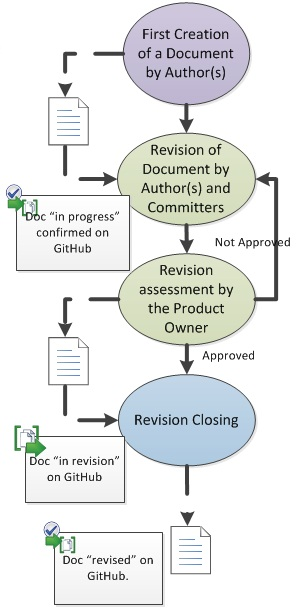
\includegraphics{./figures/RevisionProcess.JPG}
\caption{Revision-Review Processes flow}
\end{figure}


This whole process is independent from the habitual work done in the repositories; so, whereas the OpenETCS members work as usually do in the master branch, the new Revision Cycle shall be attached to a specific repository branch (previously created by the Product owner). Then any change, comment, suggestion or improvement to do to the identified document under revision, shall be done inside this RC branch and in the correspondent {\it Revision Documents} directory inside the OpenETCS structure. 

In this way, the day to day work with regard to the master branch shall not be affected by the work being done in the Revision context; the whole revision cycle for a specific document shall be linked to a specific branch of the repository. 
This is the key of the process because with this mechanism there shall be no dependencies between the ordinary work done in the project and the different Revision cycles launched for different documents at different times.

During their lifetime, these documents shall be involved at least in one complete Revision Cycle, but it there will be as many Revision Cycles as considered necessary. The different Revision Cycles linked to each document shall be numbered and associated to their branches.   

The process is divided in the following stages

\subsubsection{Document Creation Stage}

After the author(s) has completed the initial draft of a document, it must be made available to the committers involved in the Revision Process. 

The document shall be pushed into the corresponding GitHub repository in the appropriate formats (PDF, LaTex, etc).

Having the document in a format that is viewable online in GitHub provides the highest degree of access from both local and remote locations. 

The most common online formats for documents in OpenETCS project are LaTex and PDF. Each has its own advantages and, to an extent, disadvantages. 

\begin{itemize}
\item \underline{LaTex documents}
\begin{itemize}
\item They are supported by multiple opensource tools, text processors and other editing packages. 
\item It is generally easy to publish and provide access to remote users via GitHub, as well as being the most familiar format to online users.
\item LaTex provides the standard formatting and font size thanks to the use of OpenETCS Latex templates. 
\end{itemize}
\item \underline{PDF documents}
\begin{itemize}
\item The other common format is PDF. This requires the Adobe Acrobat™ software be installed on the author’s and committers PC, but provides the advantage of preserving the look and feel of the original document. 
\item PDFs are also familiar to online users and are viewable in a Web browser, although it is not possible in the GitHub context.
\end{itemize}
\end{itemize}

For this first version the \underline{Product owner} shall be clearly identified:
\begin{itemize}
\item The main author 
\item Or the project leader 
\end{itemize}

And he/she shall be the responsible for launching the Revision process and taking decisions related to the approval of the revised version of the document.

\subsubsection{Revision Stage}

The launching of the Revision process shall consist on the creation of a new {\it Revision Cycle} by the Product Owner:
\begin{itemize}
\item When starting the cycle the Revision plan and the deadline shall be clear.  
\item The Product owner shall contact the committers who have specific knowledge and appropriate experience and invite them to the process. At least, the list shall involve the committers of the project where the document is localised.
\item Identify the main contributors, at least one name shall be obtained.
\item Prepare a private e-mail for each of the identified contributors highlighting the purpose of the Revision and what is expected from his/her collaboration.
\item Specify a deadline for confirmation so the Revision Process is not delayed.
\item The Product owner shall be the responsible for addressing and conducting the main aspects of the Revision during the expected time of the cycle. 
\item The Product owner shall be aware of the progress of the Revision, so it is under control. 
\end{itemize}

The concept of the Revision stage is simple, but it can be time consuming and error prone.

Only confirmed people shall be involved in a Revision Process editing and modifying a document. They shall be registered Committers with appropriate knowledge and skills to be capable of assessing and revising a document. 

Whenever a person is required to be involved in the process and he/she is not a commiter, then a request shall be prepared by the Product owner to launch a voting process in the project. Once the person has been confirmed as a Committer, he/she can contribute in the Revision Process. Any other type of reviewers shall be involved only in the Review Process. 

The process is limited to determined number of {\it author(s)} and {\it committers} that can edit a document and push the changes to a GitHub repository. 

During the Revision process, the author(s) and committers generally benefit
from collaborating with each other, improving their productivity; and in most cases, they will convey the errors, corrections, and suggestions they want in the document. The participants in the revision shall be guided by the Product owner during the whole process so the optimum level of integration is reached. 

The conflicts that can appear due to simultaneous work in the same document shall be resolved before merging the changes into the document under Revision. So any conflict detected, question or problem found at any moment could be communicated using the {\it Issue Tracker} tool or sending an email. The Author(s) and/or the Product Manager shall be responsible for providing the appropriate support.

The revision shall be done locally by the committers/autho(s) and once they are satisfied with the changes push them to GitHub. They can use the Smartgit tool and  ensure they have switched their work context to the required RC branch. After this, then should synchronize the contents (so they have the last committed version of the document) and push their revision. The author(s) and committers can use
the todonotes package to include comments and suggestions into the document or highlight new sections or paragraphs.

When the document under revision is an intensive or complex one, the Product owner or the author(s) can propose online meetings to solve pending issues.  

When a revision is pushed to GitHub by a committer, the update shall be notified by sending a message in to the Revision team.

The stage implies the following \underline{key points}:

\begin{itemize}
\item The committers must communicate to the author(s) they have made changes to a document. 
\item Addressing the process with the use of the Smartgit tool, or any equivalent tool, to push the changes to a GitHub repository shall provide an
adequate history of the changes. At any moment there shall be available only one document and not different versions of it made by different people involved.
\item With the todonotes tool the changes made in the document should be highlighted, so any reader can identify them easily and a consistent final confirmation of changes shall be made by the Product owner. This is essential when a considerable number of committers are involved, because otherwise, the confusion becomes even greater.
\end{itemize}

At the end of the Revision Process and once the committers and author(s) are satisfied with the results, the Process owner shall be required to finally confirm and approve the version, so it can be pushed into the GitHub repository with the corresponding numbering modified.

\underline{To summarize a successful Revision cycle lies in}:
\begin{itemize}
\item The committers’ ability to communicate changes as well as their ability to collaborate together. 
\item Committers can benefit from seeing what others have done.
\item By knowing who has requested a change, and why, committers can leverage the work of one another. This prevents multiple members of the same revision team from notifying the author of the same error, or some other correction.
\item Once this process is complete, the author(s)then notify the \underline{Product owner} responsible for document the approval,the next stage in the Revision process.
\end{itemize}

\subsubsection{Approval Stage}

Now that the Revision stage is completed, the approval stage begins. 

During this stage, the \underline{Product owner} can resolve duplicate or
conflicting information and requests.

If required, more information can be requested from a committer about a
particular aspect of the revision. 

The changes made are then either confirmed or rejected with a justification.

When the changes and corrections have been accepted, then any comment made using todonotes or text highlighted shall be deleted so a clear version of the document is obtained.

\subsubsection{Closing}

The Product owner prepares the version (in LaTex and PDF) and pushed both documents to GitHub with the appropriate version numbering. 

He/she shall be also the responsible for closing the corresponding issue in the repository (if it exists) or confirming the closing via e-mail to all the author(s) and committers involved. 

He shall merge the associated RC branch into the repository {\it master branch} so the changes are officially available in the main branch of the repository.


\section{ANNEXES - Technical Instructions}

In this section the whole Revision process is explained step by step using technical instructions, so all the participants (author(s) and committers) involved in the process are aware of the mechanisms they shall implement to work and achieve the expected objectives. 

\subsection{Technical Instructions for the Product Owner}

This section includes the Technical Instructions the Product owner shall be aware of.

\subsubsection{New RC branch}

\begin{flushleft}
\tablefirsthead{}
\tablehead{}
\tabletail{}
\tablelasttail{}
\begin{supertabular}{|m{2cm}|m{13cm}|}
\hline
\rowcolor{myblue}
TI & 
TI.1.1. New RC branch
\\\hline
Roles &
Product owner
\\\hline
Description &
Any changes made to the document to be revised shall be made in a RC branch context. The Product owner shall create the branch and makes it available for the revision team.
\\\hline
Steps &
\begin{itemize}
\item Steps to create the branch locally are:
\begin{enumerate}
   \item Open Smartgit
   \item Branch menu, add branch and give a new name following this nomenclature: 
   \begin{itemize}
   \item {\it RC\_<name of the document to be revised>\_<number of Revision>}. 
   \end{itemize}
   \item Push {\it add branch \& switch}. With these steps the branch is created as a local branch.
\end{enumerate}
\item Integrate the branch into the GitHub repository
\begin{enumerate}
	\item Go to the toolbar and press {\it Push}, accept then the messages. 
	\item The new branch appears in the Smartgit Branches view, below the origin tag. 
	\item Confirm that the local branch is linked to the remote GitHub branch: in the local branch the {\it set tracked branch shall} has been done and it shall address to the RC branch already created in the GitHub repository.
\end{enumerate}
\end{itemize}
\\\hline
\end{supertabular}
\end{flushleft}

\begin{figure}[H]
\centering
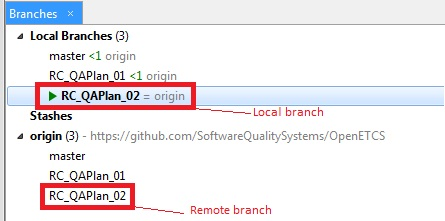
\includegraphics {./figures/Branches.JPG}
\caption{Branches tree in {\it Smartgit}}
\end{figure}

\subsubsection{Invite Committers}

\begin{flushleft}
\tablefirsthead{}
\tablehead{}
\tabletail{}
\tablelasttail{}
\begin{supertabular}{|m{2cm}|m{13cm}|}
\hline
\rowcolor{myblue}
TI & 
TI.1.2. Invite Committers
\\\hline
Roles &
Product owner
\\\hline
Description &
A new issue could be opened to contain the discussions, comments and notifications related to a specific RC for a document. Otherwise, the communications for the revision can be made privately using the e-mail and the fixed list of author(s) and committers. 
\\\hline
Steps &
\begin{itemize}
\item Create a new issue in the repository that contains the document under revision. 
\begin{enumerate}
   \item Open Github and go to the correspondent repository
   \item Select the {\it Issues section}
   \item Push the {\it New issue} button
   \item Add a descriptive title indicating the name of the new RC and the document under revision
   \item Add a significant description about the causes that have motivated the new RC and summarizes the objectives of the revision. Provide the list of required committers.
   	\item Push {\it Submit new issue}
   	\item Notify the opening of the issue to the whole revision team sending an e-mail and confirming the use of the {\it Issue tracker} to monitor the progress of the process as well as to have the discussions.
\end{enumerate}
\item Or send a private e-mail
\begin{enumerate}
   \item Add a descriptive subject indicating the name of the new RC and the document under revision
   \item Add a significant description about the causes that have motivated the new RC and summarizes the objectives of the revision. 
\end{enumerate}
\end{itemize}
\\\hline
\end{supertabular}
\end{flushleft}

\begin{figure}[H]
\centering
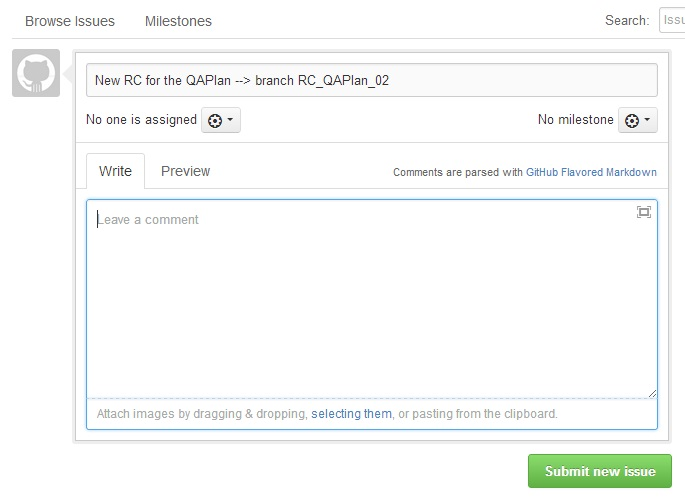
\includegraphics [width=\textwidth]{./figures/NewIssue.JPG}
\caption{New issue in {\it Github}}
\end{figure}

\subsubsection{Supervision of the Revision Process}

\begin{flushleft}
\tablefirsthead{}
\tablehead{}
\tabletail{}
\tablelasttail{}
\begin{supertabular}{|m{2cm}|m{13cm}|}
\hline
\rowcolor{myblue}
TI & 
TI.1.3. Supervision of the Revision Process
\\\hline
Roles &
Product owner
\\\hline
Description &
The Product owner shall be responsible for assessing the progress done in the RC
\\\hline
Steps &
\begin{itemize}
\item The author(s) of the document shall inform the Product owner when they and the committers have reached and agreement about the state and changes made to the document. The Product owner can read the last version available and start analyse the contents to decide whether the document shall be approved or not.
\item The Product owner shall be the responsible for updating the state of the document under revision and its backlog in the Wiki of the repository. 
\end{itemize}
\\\hline
\end{supertabular}
\end{flushleft}



\subsubsection{Final confirmation of changes}

\begin{flushleft}
\tablefirsthead{}
\tablehead{}
\tabletail{}
\tablelasttail{}
\begin{supertabular}{|m{2cm}|m{13cm}|}
\hline
\rowcolor{myblue}
TI & 
TI.1.4. Final confirmation of changes
\\\hline
Roles &
Product owner
\\\hline
Description &
The Product owner shall provide a final version with the considered changes implemented.  
\\\hline
Steps &
\begin{itemize}
\item Once the {\it Approval/rejection of comments} have been done, the changes implemented and pushed into the corresponding directory, a complete version of the document with those changes but without the comments shall be prepared.
\item The pdf and the original document shall be {\it commited} and {\it pushed} in the {\it Review Documents} directory.
\item A notification shall be included in the issue linked to the ongoing RC (if it exists) or send by e-mail: 
\begin{enumerate}
\item There, the Product owner shall explain that the changes have been implemented and that there is a complete version available in the indicated path
\end{enumerate}
\end{itemize}
\\\hline
\end{supertabular}
\end{flushleft}

\subsubsection{Revision closing}

\begin{flushleft}
\tablefirsthead{}
\tablehead{}
\tabletail{}
\tablelasttail{}
\begin{supertabular}{|m{2cm}|m{13cm}|}
\hline
\rowcolor{myblue}
TI & 
TI.1.5. Revision closing
\\\hline
Roles &
Product owner
\\\hline
Description &
The Product owner shall be the responsible for closing the current Revision Cycle after verifying and confirming all the changes done. The first task to be done is to notify the closing and highlight the results obtained.
\\\hline
Steps &
\begin{itemize}
\item Add a Comment in the Revision issue thread (if it exists) to indicate that the RC has finished
\begin{enumerate}
\item Follow the indications provided in the {\it TI.4.2 Add comments in a RC issue} to add a comment
\item Provide a brief summary of the RC:
\begin{enumerate}
\item Indicate the way the objectives have been met 
\item Are there pending objectives?. Indicate the reason for closing the RC before all the objectives have been met.
\item Identify the key aspects of the Revision
\item Highlight the results obtained
\end{enumerate}
\end{enumerate}
\item Close the RC issue thread pushing the {\it Close} button in {\it GitHub} when there is a Revision thread.
\item Or notify the closing of the RC sending an e-mail. The information included in this case is the same as before.
\end{itemize}
\\\hline
\end{supertabular}
\end{flushleft}

\subsubsection{RC Branch merging}

\begin{flushleft}
\tablefirsthead{}
\tablehead{}
\tabletail{}
\tablelasttail{}
\begin{supertabular}{|m{2cm}|m{13cm}|}
\hline
\rowcolor{myblue}
TI & 
TI.1.6. RC Branch merging
\\\hline
Roles &
Product owner
\\\hline
Description &
Merging the {\it RC Branch} to the {\it Master branch} implies incorporating the changes made in a document to the main branch of the repository. In this way, the new version of the editable document is available in the master branch.
\\\hline
Steps &
\begin{itemize}
\item Merge the branches 
\begin{enumerate}
\item Switch to the {\it master branch}, so that the working tree will be the master branch from this moment on
\item With the RC branch selected the Product owner shall do a click on the right button and select {\it merge to working tree}.
\end{enumerate}
\item Confirm the update
\begin{enumerate}
\item Make {\it push} to the repository and the merge shall be done.
\item Make {\it synchronize} so all the changes made are reflected remotely and locally.
\end{enumerate}
\end{itemize}
\\\hline
\end{supertabular}
\end{flushleft}

\subsection{Technical Instructions for the Author(s)}

This section includes the Technical Instructions the Author(s) shall be aware of.

\subsubsection{Approval/rejection of comments}

\begin{flushleft}
\tablefirsthead{}
\tablehead{}
\tabletail{}
\tablelasttail{}
\begin{supertabular}{|m{2cm}|m{13cm}|}
\hline
\rowcolor{myblue}
TI & 
TI.2.1. Approval/rejection of comments
\\\hline
Roles &
Author(s)
\\\hline
Description &
The Author(s) shall study each proposal, recommendation or comment that appears in the document under revision and decide how to implement the proposed changes in case he/she estimates it is appropriate to be included in the document. On the other hand, and considering the committers could include text in the document, the author(s) shall assess the appropriateness of those sections and decide if this new content is accurate and relevant. 
\\\hline
Steps &
\begin{itemize}
\item When a committer notifies that some changes have been pushed to GiThub using the corresponding RC branch, the Author(s) synchronizes their repository to obtain the last commit made for the document with the {\it SmartGit} tool.
\item The Author(s) reads carefully any annotation that appears in the document and decides whether the comments shall be implemented or not.
\item For each annotation the Author(s) find(s) in the document, a written confirmation about what is the decision about the subject shall be provided. 
\begin{enumerate}
\item Use the {\it todonotes} to confirm/reject proposals made by the Committers ({\it TI.4.2 Add notes using todonotes}) or to accept/delete new sections, text or paragraphs added by the committers.
\item In any case, a justification for that decision shall be included.
\item When a suggestion is accepted:
\begin{enumerate}
\item Assess whether the recommendation made implies writing new paragraphs, sections, adding new figures, etc. and modify the document accordingly. 
\item Highlight the new text or the modified text with {\it todonotes} using the {\it inline} option.
\end{enumerate}
\end{enumerate}
\item The Author(s)commits the changes made in the document and push them into the RC branch so the committers can have access to the changes, confirmations and rejections made by the Author(s).
\item The Author(s) add(s) a message to the RC issue thread (if it exists) or send(s) an e-mail, so everyone can be informed about the commit recently done. 
\end{itemize}
\\\hline
\end{supertabular}
\end{flushleft}

\begin{figure}[H]
\centering
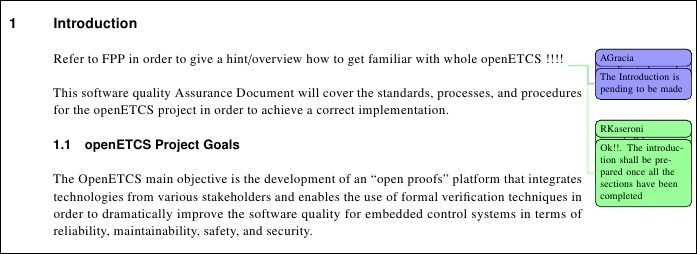
\includegraphics [width=\textwidth]{./figures/CommentConfirmation.JPG}
\caption{Using todonotes package Accept/Reject changes {\it Github}}
\end{figure}

\subsection{Technical Instructions for the Committers}

This section includes the Technical Instructions the Committers shall be aware of.

\subsubsection{Revision Environment setup}

\begin{flushleft}
\tablefirsthead{}
\tablehead{}
\tabletail{}
\tablelasttail{}
\begin{supertabular}{|m{2cm}|m{13cm}|}
\hline
\rowcolor{myblue}
TI & 
TI.3.1. Revision environment setup
\\\hline
Roles &
Committers
\\\hline
Description &
Each Committer shall prepare the working environment locally and ensure it is ready before starting with the Revision tasks.
\\\hline
Steps &
\begin{itemize}
\item Setup using {\it Smartgit} tool
\begin{enumerate}
\item Clone the repository with the {\it Project --> Clone} option.
\item Go to the {\it Branch} menu, select {\it Add branch} and give a name. Then, the branch is created as a local branch.
\item Link the local branch to the remote git branch, to do that, select {\it Set tracked branch} in the context menu of the local branch. The local environment is then ready for working in the Revision Process
\end{enumerate}
\item Update the environment
\begin{itemize}
\item It is essential to work in the last version of the document under Revision, so minimal conflicts appear in the future when uploading the changes. To be sure about this, a pull request shall be done to the repository before editing the document.
\begin{itemize}
\item Select the {\it Pull} option on the toolbar
\end{itemize}
\end{itemize}
\end{itemize}
\\\hline
\end{supertabular}
\end{flushleft}

\subsubsection{Revision work}

\begin{flushleft}
\tablefirsthead{}
\tablehead{}
\tabletail{}
\tablelasttail{}
\begin{supertabular}{|m{2cm}|m{13cm}|}
\hline
\rowcolor{myblue}
TI & 
TI.3.2 Revision work
\\\hline
Roles &
Committers
\\\hline
Description &
The Committers shall perform the revision in the expected time and conditions. The work of a committer shall finish when the Product owner confirms the closing of the RC.
\\\hline
Steps &
\begin{itemize}
\item The Committer shall:
\begin{enumerate}
\item Make comments, suggestions or improvement proposals with the {\it todonotes} (See {\it TI.4.1 Add notes using todonotes}).
\item Add comments in the RC issue thread when it applies (See {\it TI.4.2 Add comments in a RC issue}).
\item Make changes in the document. Each insertion shall be highlighted indicating the initials of the person involved. The Revision process shall be done by different people and what comments have been written by whom shall be known.
\end{enumerate}
\item The Committer shall integrate the changes into the document that is hosted in the remote repository in GitHub. 
\item To do that, click on the {\it Push} button in the SmartGit tool. When pushing different situations can happen:
\begin{itemize}
\item There are no conflicts with the original repository .
\begin{enumerate}
\item The changes shall be included.
\end{enumerate}
\end{itemize}
\begin{itemize}
\item There are one or more conflicts.
\begin{enumerate}
\item Click on the {\it Pull} button so the last version is loaded. 
\item Open the {\it Conflict Solver} Window to compare the committed version in the {\it Github} and the local version. 
\item The conflict shall be solved in the following way.
\begin{enumerate}
\item The Committer shall indicate that the version stored in the remote repository is the correct one. The changes in case of conflict are not included. 
\item The Committer will {\it Commit} and {\it Push} the changes that do not have any conflict and add a notification in the document about that. 
\item After finishing the {\it pushing}, he/she shall perform a {\it pulling} to obtain the integrated and last committed version; then he/she shall add a note using {\it todonotes} tool in the section where the conflicts were; he/she shall explain the problem found. 
\end{enumerate}
\item Have in mind that after {\it pushing/pulling} the document, the changes in conflict made by the Committer shall be lost. Anytime a conflict appears, the Committer shall prepare a copy of the suggestions or modifications made by him/her.
\item He/she also adds a comment in the RC issue thread (if it exists) or send an e-mail exposing that problem and requesting a solution.
\item The Author(s) and(or the Product owner shall take part in the discussion and propose a solution. The Committer can put in the document again the suggestions in conflict stored locally if the Author(s) or the Product owner requires that.
\end{enumerate}
\end{itemize}
\end{itemize}
\\\\\hline
Steps &
\begin{itemize}
\item In any case, the Committer shall inform about the progress of the work posting a message in the RC issue thread or sending an e-mail. (See {\it TI.4.2 Add comments in a RC issue}).
\end{itemize}
\\\hline
\end{supertabular}
\end{flushleft}

\begin{figure}[H]
\centering
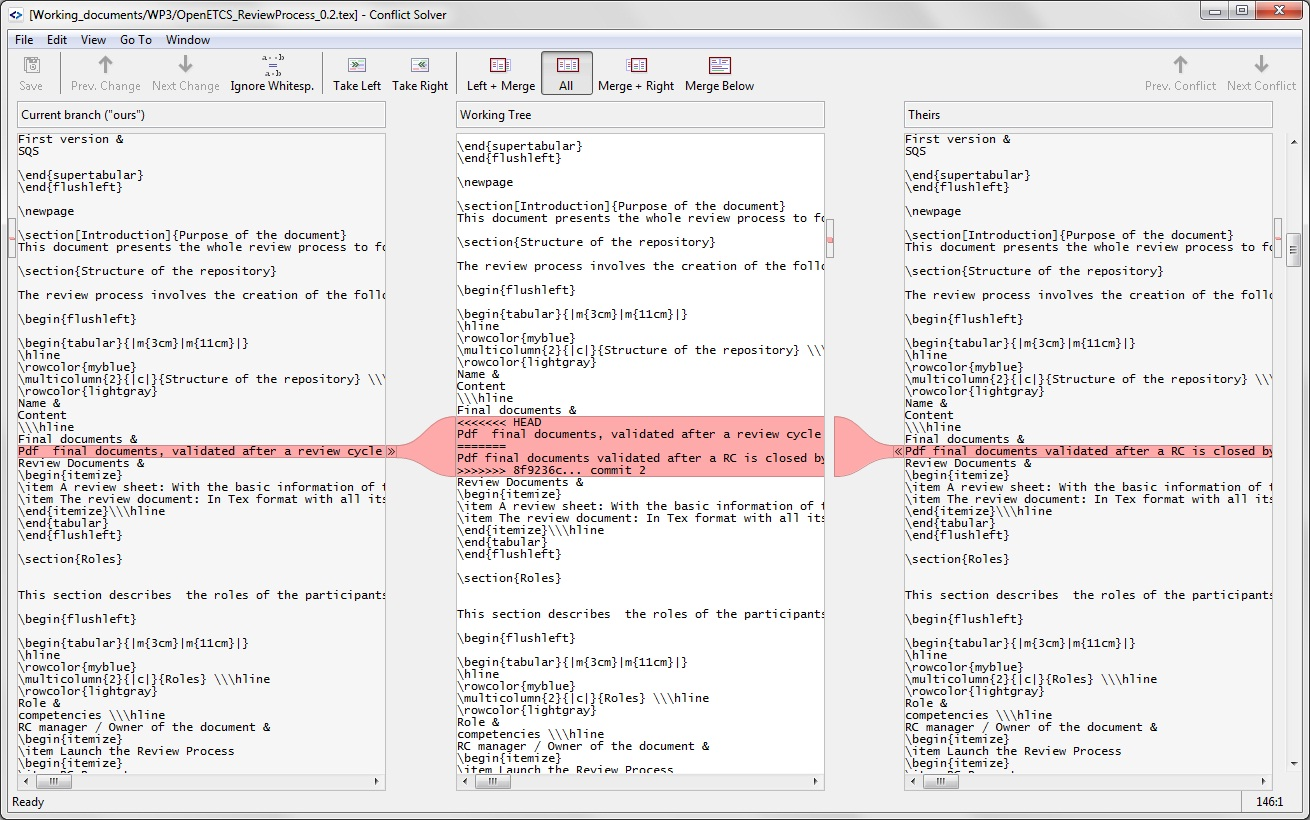
\includegraphics[width=\textwidth]{./figures/ConflictSolverWindow.JPG}
\caption{Conflict Solver Window}
\end{figure}

\subsection{Technical Instructions for any Role}
This section includes any Technical Instruction that shall be followed by the Product owner, the Author(s) or the Committers at different phases of the Revision Process

\subsubsection{Add notes using todonotes}

\begin{flushleft}
\tablefirsthead{}
\tablehead{}
\tabletail{}
\tablelasttail{}
\begin{supertabular}{|m{2cm}|m{13cm}|}
\hline
\rowcolor{myblue}
TI & 
TI.4.1 Add notes using todonotes
\\\hline
Roles &
Product Owner, Author(s), Committers
\\\hline
Description &
The package todonotes must be installed locally to make comments in the document under Revision. 
\\\hline
Steps &
\begin{itemize}
\item Verify the installation of the todonotes package locally. In case the package is not installed, follow these steps:
\begin{enumerate}
\item Got to the {\it MixTex} tool directory, select {\it Maintenance (Admin)} and click on {\it Package Manager (Admin)}.
\item Look for the {\it todonotes} package using the filtering option.
\item Select the package after the search is done and install.
\end{enumerate}
\item Be used to the most common commands available in the package.
\begin{enumerate}
\item Go to the {\it governance} repository in the Github and look for the {\it Reviews Process} folder. There you can find a {\it todonotes} document that explains all the commands that can be used during the reviewing.
\end{enumerate}
\item Identify always any comment done with your initials.
\begin{enumerate} 
\item The initials of the person who inserts a comment into the document shall be the the first letter of the name plus the surname.
\end{enumerate}
\item Use different colours in the document for different meanings 
\begin{enumerate}
\item {\it Red}: indicate in a comment what paragraph, section or line is proposes to be deleted. 
\item {\it Green}: the suggestion made by has been approved.
\item {\it Orange}: the comment refers to any conflict found between commits done by different people. It also shall be used when commentign a suggestions that shall be discussed and not implemented for the moment.
\item {\it Yellow}: any general comment done by the participants in the Revision. 
\end{enumerate} 
\end{itemize}

\\\hline
\end{supertabular}
\end{flushleft}

\subsubsection{Add comments in a RC issue}

\begin{flushleft}
\tablefirsthead{}
\tablehead{}
\tabletail{}
\tablelasttail{}
\begin{supertabular}{|m{2cm}|m{13cm}|}
\hline
\rowcolor{myblue}
TI & 
TI.4.2 Add comments in a RC issue
\\\hline
Roles &
Product owner, Author(s), Committers
\\\hline
Description &
The issue opened by the Product owner at the beginning of the RC shall be used whenever a notification shall be done, conflict reported or questions asked. The collaborative work shall aim to get a dynamic approach when the discussions are fluid, with quick answers and sharing of information.
\\\hline
Steps &
\begin{itemize}
\item Go to the repository where the document under Revision is located.
\item Select the issue that has the RC you are working on.
\item The comments posted shall be descriptive enough so any reader can understand the message. 
\begin{enumerate}
\item Identified yourself clearly, providing your name and role in the project.
\item When required, include diagrams, figures, partial texts or specific data that help to understand the problematic found.
\end{enumerate}
\item Do not edit any comment done. It is a better option to rewrite it with the additions you proposed than editing and make the changes directly. In this way, it is assured that everyone reads the new message because in the other case, the change/addition can be missed.
\item Push the {\it Comment} button to post the message.
\end{itemize}

\\\hline
\end{supertabular}
\end{flushleft}

\end{document}
